\chapter[Introduction]{Introduction}
\label{chap:introduction}

We all want software to run fast and efficiently. 
Software performance severely affects usability of software system,
and it is one of the most important problems in computer science research. 
Performance bugs are one major source of software's slowness and inefficiency. 
Performance bugs are software implementation mistakes that can cause inefficient execution. 
Due to their non fail-stop symptoms, 
performance bugs are easy to escape from in-house testing and difficult to be diagnosed. 
Nowadays, the urgency to address performance bugs is becoming even more important 
with new hardware and software trends and increasing concerns about energy constraints. 

Facing the challenge of performance bugs, 
this dissertation proposes effective performance-bug detection 
and performance-bug diagnosis approaches based on a 
comprehensive characteristics study of real-world performance bugs.

\section{Motivation}
Slow and inefficient software can easily frustrate users and
cause financial losses.
Although researchers have devoted decades to
transparently improving software performance,
{\it performance bugs} continue to pervasively
degrade performance
and waste computation resources in the field~\citep{rily.perftest}.
Meanwhile, current support for combating performance bugs is preliminary due
to the poor understanding of real-world performance bugs.

Following the convention of developers and researchers 
on this topic~\citep{s2e,perf.fse10,rily.perftest,perfantipattern},
we refer to performance bugs
%~\footnote{We will use performance bugs
%and performance problems interchangeably in this thesis following previous work in this 
%area~\citep{Alabama,perf.fse10}.} 
as software defects, which can slow down the program.
Relatively simple {\it source-code} changes can fix performance bugs, 
and significantly speed up software, 
while preserving functionality.
These defects can{\bf not} be optimized away by state-of-practice compilers,
thus bothering end users.

%\begin{figure}
%\codefig{Apache45464}
%\caption{A performance bug from Apache-HTTPD
%  {(`+' and `-' denote the 
%    code added and deleted to fix this bug)}}
%\label{fig:Apache45464}
%\end{figure}

\begin{figure}
\codefig{GCC27733}
\caption{A real-world performance bug in GCC (the `-' and `+' demonstrate the patch)}
\label{fig:GCC27733}
\end{figure}

%Figure~\ref{fig:Apache45464} shows an example of a real-world performance bug. 
%Apache HTTPD developers forgot to change a parameter of API \Code{apr_stat} after an API upgrade. 
%This mistake causes \Code{apr_stat} to retrieve more than necessary information 
%from the file system and leads to more than ten times slowdown in Apache server. 
%After changing to \Code{APR_FINFO_TYPE}, \Code{apr_stat} will retrieve exactly what 
%developers originally needed through \Code{APR_FINFO_NORM}. 

Figure~\ref{fig:GCC27733} shows an example of a real-world performance bug.
A small mistake in the type declaration of hash-table entry \texttt{alg\_hash\_entry} 
causes the designed memoization for \texttt{synth\_mult} not to work, when \texttt{t}
is larger than the maximum value type-\texttt{int} can represent. 
As a result, under certain workload, \texttt{synth\_mult} conducts a lot of
redundant computation for same \texttt{t} values repeatedly, 
leading to 50 times slowdown. 

Performance bugs exist widely in released software. 
For example, Mozilla developers have fixed 5--60 performance bugs
reported by users {\it every month} over the past 10 years.
The prevalence of performance bugs is inevitable because
little work has been done to help developers avoid
performance-related mistakes. In addition,
performance testing mainly relies on ineffective black-box random 
testing and manual input design, which allows the majority of performance bugs
to escape~\citep{rily.perftest}.

Performance bugs lead to reduced throughput, increased latency, and 
wasted resources in the field. 
In the past, they have caused several 
highly publicized failures, causing hundred-million dollar software 
projects to be abandoned~\citep{colorado,uk}.

Worse still, performance problems are costly to 
diagnose due to their non fail-stop symptoms.
Software companies may need several months of effort by experts
to find a couple of performance bugs that cause a few 
hundred-millisecond delay in
the 99th percentile latency of their service~\citep{dicksites}.

The following trends will make the performance-bug problem more critical
in the future:

{\bf Hardware:} For many years,  
  Moore's law ensured that hardware would make software faster over time 
  with no software
  development effort. In the multi-core era, when each core is unlikely to 
  become faster, performance bugs are particularly harmful.

{\bf Software:} The increasing complexity of software systems and rapidly 
changing workloads provide new opportunities for performance waste and
new challenges in diagnosis
\citep{BloatFSE2008}.
Facing the increasing pressure on productivity, 
developers cannot combat performance bugs without automated tool support. 

{\bf Energy efficiency:} 
Increasing energy costs provide a powerful economic 
argument for avoiding performance bugs. 
When one is willing to sacrifice the service quality to reduce 
energy consumption~\citep{green.pldi10,asplos11karthik}, 
ignoring performance bugs is unforgivable.
For example, by fixing bugs that have doubled the
execution time,
one may potentially
halve the carbon footprint of buying and operating computers.

Performance bugs may not have been reported as often as functional bugs, because 
they do not cause fail-stop failures.
However, considering the preliminary support for
combating performance bugs,
it is time to pay more attention to them, 
when we enter a new resource-constrained computing world.

\section{Thesis philosophy}

The topic of this thesis is to provide better tool support to combat performance bugs. 
The philosophy of this thesis is to investigate existing approaches originally designed for 
functional bugs,
%~\footnote{Any software defects that lead to functional misbehavior,
%such as incorrect outputs, crashes, and hangs. They include
%semantic bugs, memory bugs, concurrency bugs, and others.} , 
and try to apply, adapt, and extend them for performance bugs. 

This philosophy is promising, 
because many advanced techniques have been proposed for functional bugs in each stage of software development. 
For example, many detection tools~\citep{chouasplos00,billpugh,PRMiner05,semanticpatch,fortify} 
can help point out previously unknown functional bugs, 
automated testing tools~\citep{KLEE,s2e} can exercise software under different setting 
or inputs and expose functional problems, 
and there are also diagnosis~\citep{liblit03, liblit05, CCI} and 
fixing tools~\citep{afix, ofix, mfix} for reported functional bugs.

There are also uncertainties behind this philosophy. 
For example, in order to build effective performance-bug detection techniques, 
we need to know what are common root causes for performance bugs, 
which are not obvious, due to the poor understanding of real-world
performance bugs. 
For example, many functional failure diagnosis techniques
highly depend on failure symptoms, like crashes. 
Unfortunately, performance
bugs have non fail-stop symptoms, and it is even unclear how to identify failure
runs for performance bugs.

\begin{table}[t!]
\centering
\scriptsize
\begin{tabular}{@{\hspace{3pt}}l@{\hspace{3pt}}@{\hspace{3pt}}c@{\hspace{3pt}}@{\hspace{3pt}}c@{\hspace{3pt}}}
\toprule
Techniques in this thesis                &    Functional Bug    &   Performance Bug     \\
\midrule                            
{\bf Rule-based bug detection} 	         &      \checkmark      & \checkmark            \\
\midrule                            
{\bf Statistical debugging}              &      \checkmark      & \checkmark\\
\midrule
{\bf Sampling-based approach }           &     \checkmark       &  \checkmark \checkmark\\
\midrule
{\bf LDoctor}                            &      \ding{55}                & \checkmark\\
\bottomrule
\end{tabular}
\caption{Techniques in this thesis}
\label{tab:1_technique}
\end{table}



Following techniques are explored and extended for performance bugs in this thesis. 
All of these techniques are previously designed for functional bugs.

{\bf Rule-base bug detection:}
There are many correctness rules inside software. 
For instance, lock has to be followed by an unlock, 
opened files must be closed, and allocated memory must be freed. 
Violations to these rules may lead to critical system failures. 
Many techniques~\citep{chouasplos00,billpugh,PRMiner05,semanticpatch,fortify,WOODPECKER} 
are designed to detect rule-violations 
and identify previously unknown bugs.
In this thesis, we find that there are also statically checkable efficiency-related rules in software, 
and violating them would lead to inefficient computation.
These rules can be leveraged to detect previously unknown performance bugs, 
as shown by the first row in Table~\ref{tab:1_technique}. 

{\bf Statistical Debugging:}
Statistical debugging~\citep{liblit03,liblit05,CCI,tarantula1,tarantula2,tarantula.darko,joy.asplos13} 
is one of the most effective failure diagnosis techniques. 
It usually works in two steps. 
First, a set of run time events, referred to as predicates, are collected from both success runs and failure runs.
Second, statistical models are used to identify predicates that are highly correlated with failure. 
In this thesis, we find that after selecting right types of predicates and statistical models, 
statistical debugging is effective for providing coarse-grained root-cause information for performance bugs, 
as shown by the second row in Table~\ref{tab:1_technique}. 
This finding also motivates us to develop a tool, {\bf LDoctor}, 
dedicated for identifying fine-grained root causes for performance bugs, as shown by the fourth row in Table~\ref{tab:1_technique}.

{\bf Sampling-based approach:}
Sampling-based techniques~\citep{liblit03,liblit05,CCI,joy.asplos13} collect predicates from production runs in a low overhead. 
Since less information is collected in one single run, 
sampling-based approaches usually rely on multiple runs to achieve the same diagnosis capability, 
sacrificing diagnosis latency. 
In this thesis, we find that sampling can keep the capability of statistical performance diagnosis, 
while lowering the runtime overhead. 
Since root-cause related predicates usually appear multiple times in one performance failure run, 
sampling works better for performance bugs than functional bugs, 
as shown by the third row in Table~\ref{tab:1_technique}. 

\section{Dissertation Contribution}


\begin{figure}[t!]
\begin{center}
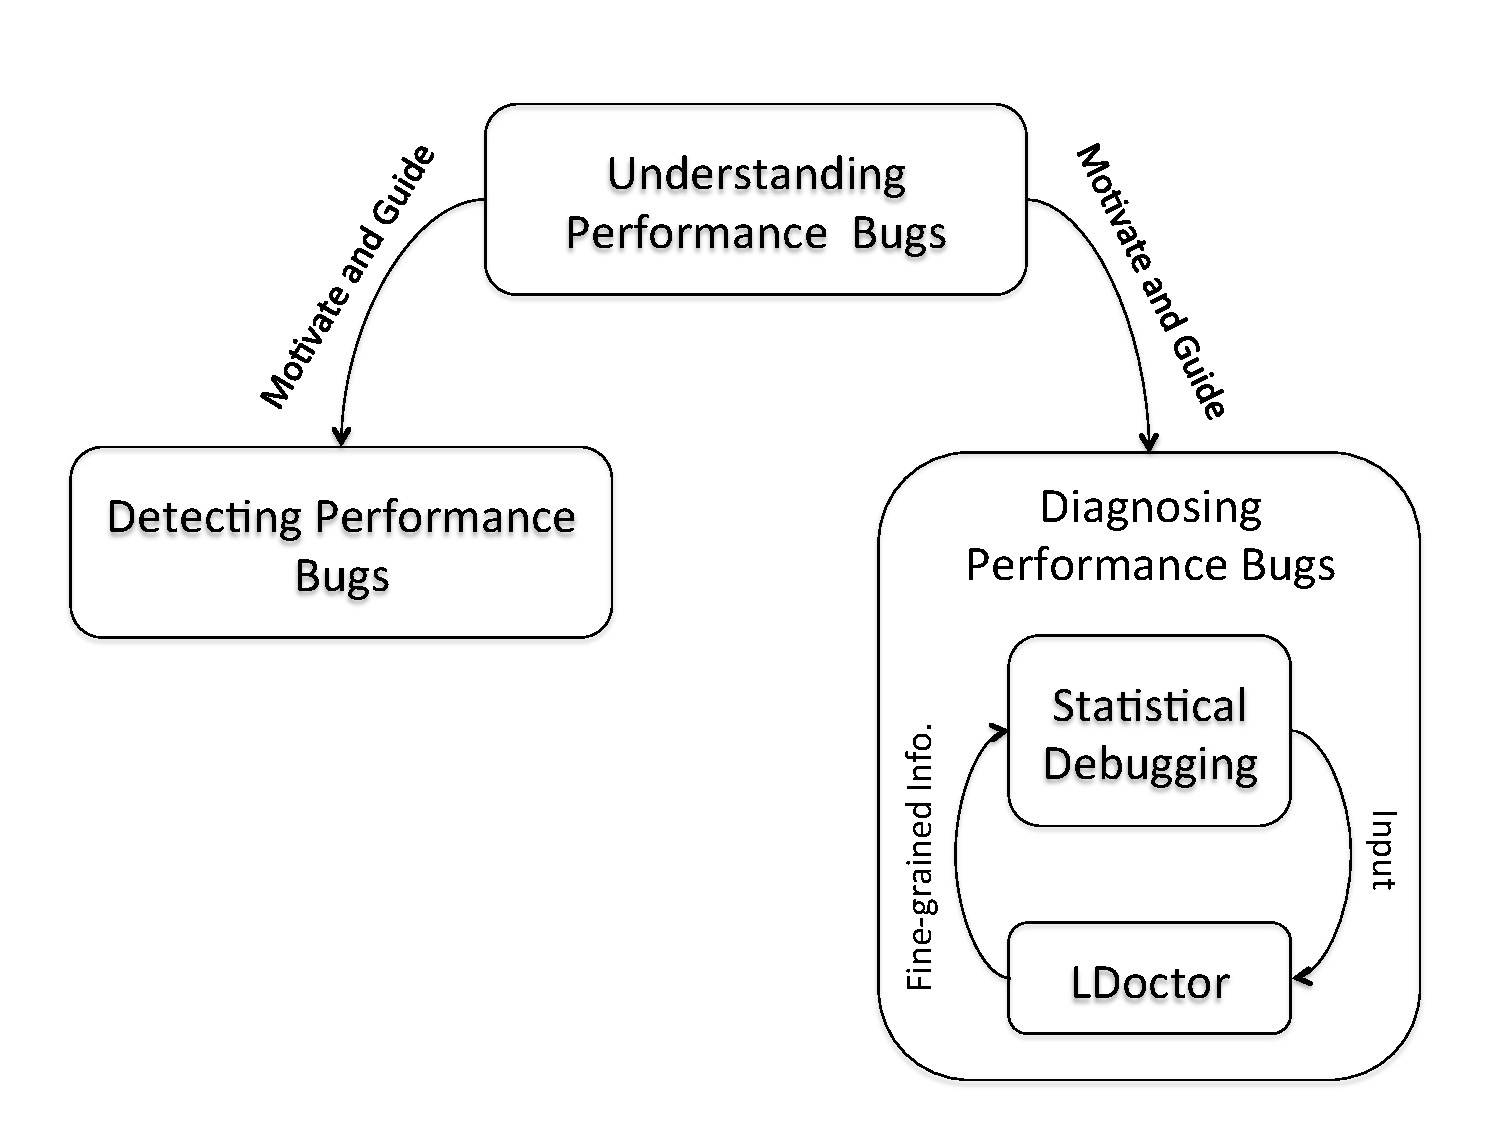
\includegraphics[width=4.5in]{figures/overview}
\caption{Interactions among the four components in this dissertation.}
\label{fig:overview}
\end{center}
\end{figure}

This dissertation works on three directions to address performance-bug problems:
real-world performance-bug understanding, 
performance-bug detection and performance failure diagnosis. 
%Specifically, we conduct the first empirical study on real-world performance bugs. 
%Our study can guide future research on performance bugs, and 
%it has already inspired our own detection and diagnosis work. 
%We examine final patches of fixed performance bugs, extract rules from these patches, 
%and build checkers to detect violations to these rules. 
%We explore the feasibility and design space to apply statistical debugging to performance failure diagnosis. 
%By leveraging different statistical models, 
%statistical debugging can identify buggy branches, which are taken only during performance failure runs, 
%or inefficient loops, which execute more iterations during performance failure runs. 
%We think localizing inefficient loops is not informative enough for performance diagnosis.
%Therefore, we build LDoctor, which is a series of static-dynamic hybrid analysis for identified inefficient loops from statistical debugging. 
%LDoctor can provide root-cause information and fix suggestions to developers. 
The components in this dissertation interact and complement each other as shown in Figure~\ref{fig:overview}.

%Techniques involved in this thesis are shown in Table~\ref{tab:1_technique}. 
%Rule-based bug detection and statistical debugging work for both functional bugs and performance bugs. 
%Sampling works better for performance bugs, 
%because failure root causes appear more than once in one performance failure run. 
%LDoctor is a technique designed for performance bugs.

\subsection{Understanding performance bugs}

Addressing performance bug problems require approaches from different aspects, 
and all these aspects will benefit from a better understanding of performance bugs. 

This dissertation conducts a comprehensive characteristics study on 
a large number of real-world performance bugs collected from five widely used large open-source applications: 
Apache, Chrome, GCC, Mozilla and MySQL. 
This study reveals many interesting findings about performance bugs' root-cause patterns, 
how performance bugs are introduced, performance bugs' manifestation conditions, and fix strategies. 
It directly motivates performance-bug detection work and performance-bug diagnosis work in this thesis. 

\subsection{Rule-based performance-bug detection}

Guided by our characteristics study, we hypothesize that 
(1) efficiency-related rules exist; 
(2) we can extract rules from performance-bug patches; 
and (3) we can use the extracted rules to discover previously unknown performance bugs. 
To test these hypotheses, we collect rules from 25 Apache, Mozilla, and MySQL bug patches 
and build static checkers to find violations to these rules.

Our checkers find 332 previously unknown Potential Performance Problems (PPPs) 
in the latest Apache, Mozilla, and MySQL. 
These include 219 PPPs found by checking an application using rules extracted from a different application. 
Our thorough code reviews and unit testings confirm that each PPP runs significantly slower 
than its functionality-preserving alternate suggested by the checker. 
We report some of found PPPs to developers. 
77 PPPs are already confirmed by developers and 15 PPPs are fixed.  

The main contribution of our bug-detection work is that it 
confirms the existence and value of efficiency rules: 
efficiency rules in our study are usually violated at more than one place, 
by more than one developer, 
and sometimes in more than one program. 
Rule-based performance-bug detection is a promising direction. 

\subsection{Statistical debugging for real-world performance bugs}
Statistical debugging is one of the most effective failure diagnosis techniques proposed for functional bugs. 
We explore whether it is possible to apply statistical debugging to performance bugs, 
and how to apply statistical debugging to performance bugs. 

We first conduct an empirical study to understand how performance problems are observed and reported by real-world users. 
Our study shows that statistical debugging is a natural fit for diagnosing performance bugs, 
which are often observed through comparison-based approaches and reported together with both good and bad inputs. 
We then thoroughly investigate different design points in statistical debugging, 
including three different predicates and two different types of statistical models, 
to understand which design point works the best for performance diagnosis. 
Finally, we study how some unique nature of performance bugs allows sampling techniques 
to lower the overhead of runtime performance diagnosis without extending the diagnosis latency. 

\subsection{Performance diagnosis for inefficient loops}
Statistical debugging can accurately identify control-flow constructs, like branches or loops,
that are most correlated with the performance problem by comparing problematic runs and regular runs. 
Unfortunately, for loop-related performance bugs, which contribute to
two thirds of real-world user-perceived performance bugs in our study, 
these coarse-grained root-cause information is not enough.
Although statistical debugging can identify the root-cause loop, it does
not provide any information regarding why the loop is inefficient 
and hence is not very helpful in fixing the performance bug.


In order to provide fine-grained root-cause information, we design LDoctor, 
which is a series of static-dynamic hybrid analysis, for inefficient loops. 
We build LDoctor through two steps. 
The first step is to figure out a taxonomy of the root causes for common inefficient loops. 
The second step is to follow the taxonomy and design analysis for each root-cause subcategory. 
In order to balance accuracy and performance, we hybridize static and dynamic analysis. 
We further use sampling to lower the runtime overhead. 
Evaluation using real-world performance bugs shows that LDoctor can provide good coverage and accuracy, 
with small runtime overhead.

\section{Dissertation Outline}
The remainder of this dissertation is organized as follows. 
\Cref{chap:background} describes previous work on characteristics study of performance bugs, 
performance-bug detection, performance failure diagnosis, and other related topics. 
\Cref{chap:study} presents our characteristics study of real-world performance bugs. 
\Cref{chap:detec} focuses on our rule-based performance-bug detection work. 
\Cref{chap:sd} explains our work about exploring how to apply statistical debugging to performance failure diagnosis. 
\Cref{chap:ldoctor} discusses LDoctor, which can effectively diagnose inefficient loops. 
